\subsection{Merkmalsextraktion}
\label{merkmalsextraktion}

Die Darstellung eines Bildes über einen Graphen \gls{G}, der aus einer Superpixelrepräsentation \gls{Smenge} gewonnen wurde, besitzt in der Regel weitaus weniger Knoten im Gegensatz zu der reinen Darstellung des Bildes über eine Gitterrepräsentation.
Die Superpixel \bzw{} die Regionen der Segmentierungsmaske können dabei jedoch die willkürlichsten Formen annehmen und besitzen lediglich die Einschränkung, dass diese stets zusammenhängend sind.
Die Form eines Superpixels muss demnach bestmöglichst eingefangen \bzw{} beschrieben werden können — ein Prozess, der in der Bildverarbeitung als \emph{Merkmalsextraktion} bekannt ist~\cite{momente}.
Ein geeigntes Mittel zur Beschreibung einzelner Objekte in einem segmentierten Bild sind die \emph{Momente}, welche in nicht-zentrierte, translationsinvariante, skalierungsinvariante und rotationsinvariante Momente unterschieden werden~\cite{momente}.

\paragraph{Nicht-zentrierte Momente}
\label{nicht_zentrierte_momente}

Zu der binären Segmentierungsmaske $\gls{Smaske} \in {\left\{0, 1\right\}}^{H \times W}$ sind die \emph{nicht-zentrierten Momente} vom Grad $\left(i+j\right)$, $i,j\in\gls{N}$, definiert als~\cite{momente}
\begin{equation*}
  \gls{M}_{ij} \coloneqq \sum_x^W \sum_y^H x^i y^j \gls{Smaske}_{yx}.
\end{equation*}
Obwohl der Grad eines Moments beliebig hoch gewählt werden kann, so reichen in der Praxis meist wenige Momente niedrigen Grades aus ($\le 3$), um eine Region hinreichend genau zu charakterisieren~\cite{momente}.
Bildeigenschaften, die durch nicht-zentrierte Momente beschrieben werden können, sind unter anderem dessen Fläche über $\gls{M}_{00}$ sowie dessen absoluter Schwerpunkt $\left\{\bar{x}, \bar{y}\right\} = \left\{ \gls{M}_{10}/\gls{M}_{00}, \gls{M}_{01}/\gls{M}_{00}\right\}$~\cite{momente}.

\paragraph{Translationsinvariante (zentrale) Momente}
\label{translationsinvariante_momente}

Nicht-zentrierte Momente sind aufgrund ihrer Berücksichtigung der Position einer Region im Bild meist unerwünscht, sie helfen aber für die weitere Definition von translationsinvarianten Momenten.
Mit Hilfe der absoluten Schwerpunktskoordinaten $\left\{ \bar{x}, \bar{y} \right\}$ können die \emph{translationsinvarianten Momente} über
\begin{equation*}
  \gls{mu}_{ij} \coloneqq \sum_x^W \sum_y^H {\left(x - \bar{x}\right)}^i {\left(y - \bar{y}\right)}^j \gls{Smaske}_{yx}.
\end{equation*}
definiert werden~\cite{momente}.
Sie lassen sich weiterhin direkt aus $\gls{M}_{ij}$ ermitteln.
So gilt \zB{}, dass $\gls{mu}_{00} = \gls{M}_{00}$ oder $\gls{mu}_{11} = \gls{M}_{11} - \bar{x}\gls{M}_{01} = \gls{M}_{11} - \bar{y}\gls{M}_{10}$ (\vgl{}~\cite{momente}).

\paragraph{Skalierungsinvariante Momente}
\label{skalierungsinvariante_zentrierte_momente}

Für $i+j \geq 2$ können desweiteren die \emph{skalierungsinvarianten Momente} $\gls{eta}_{ij}$ konstruiert werden, die invariant \bzgl{} Skalierung und Translation sind.
Dafür wird das entsprechende translationsinvariante Moment $\gls{mu}_{ij}$ durch die entsprechende Fläche $\gls{M}_{00}$ \bzw{} $\gls{mu}_{00}$ des Segments geteilt, \dhe{}~\cite{momente}
\begin{equation*}
  \gls{eta}_{ij} = \frac{\gls{mu}_{ij}}{\gls{mu}_{00}^{\left(1+\left(i+j\right)/2\right)}}.
\end{equation*}

\paragraph{(Rotationsinvariante) Hu-Momente}
\label{rotationsinvariante_momente}

\citeauthor{Hu} verwendet eine nichtlineare Kombination der skalierungsinvarianten Momente bis zum Grad $3$, um aus ihnen zusätzlich eine Rotationsinvarianz zu gewinnen~\cite{Hu, momente}.
Daraus ergeben sich die sieben \emph{rotationsinvariante Momente} \bzw{} die \emph{Hu-Momente}~\cite{momente}.
\begin{equation*}
\begin{split}
  \gls{hu}_1 & = \gls{eta}_{20} + \gls{eta}_{02}\\
  \gls{hu}_2 & = {\left(\gls{eta}_{20} - \gls{eta}_{02}\right)}^2 + {\left(2\gls{eta}_{11}\right)}^2\\
  \gls{hu}_3 & = {\left(\gls{eta}_{30} - 3\gls{eta}_{12}\right)}^2 + {\left(3\gls{eta}_{21} - \gls{eta}_{03}\right)}^2\\
  \gls{hu}_4 & = {\left(\gls{eta}_{30} + \gls{eta}_{12}\right)}^2 + {\left(\gls{eta}_{21} + \gls{eta}_{03}\right)}^2\\
  \gls{hu}_5 & = \left(\gls{eta}_{30} - 3\gls{eta}_{12}\right)\left(\gls{eta}_{30} + \gls{eta}_{12}\right) \left({\left(\gls{eta}_{30} + \gls{eta}_{12}\right)}^2 - 3{\left(\gls{eta}_{21} + \gls{eta}_{03}\right)}^2\right)\\
  & + \left(3\gls{eta}_{21} - \gls{eta}_{03}\right)\left(\gls{eta}_{21} + \gls{eta}_{03}\right) \left(3{\left(\gls{eta}_{30} + \gls{eta}_{12}\right)}^2 - {\left(\gls{eta}_{21} + \gls{eta}_{03}\right)}^2\right)\\
  \gls{hu}_6 & = \left(\gls{eta}_{20} - \gls{eta}_{02}\right)\left({\left(\gls{eta}_{30} + \gls{eta}_{12}\right)}^2 - {\left(\gls{eta}_{21} + \gls{eta}_{03}\right)}^2\right) + 4\gls{eta}_{11}\left(\gls{eta}_{30} + \gls{eta}_{12}\right)\left(\gls{eta}_{21} + \gls{eta}_{03}\right)\\
  \gls{hu}_7 & = \left(3\gls{eta}_{21} - \gls{eta}_{03}\right)\left(\gls{eta}_{30} + \gls{eta}_{12}\right) \left({\left(\gls{eta}_{30} + \gls{eta}_{12}\right)}^2 - 3{\left(\gls{eta}_{21} + \gls{eta}_{03}\right)}^2\right)\\
  & + \left(\gls{eta}_{03} - 3\gls{eta}_{12}\right)\left(\gls{eta}_{21} + \gls{eta}_{03}\right) \left(3{\left(\gls{eta}_{30} + \gls{eta}_{12}\right)}^2 - {\left(\gls{eta}_{21} + \gls{eta}_{03}\right)}^2\right)
\end{split}
\end{equation*}

\paragraph{Weitere Merkmale}
\label{weitere_merkmale}

Aus den translationsinvarianten Momenten lassen sich weitere Merkmale gewinnen, denen insbesondere eine anschauliche Interpretation zu Grunde liegt.
Sei dafür die \emph{Kovarianzmatrix} der binären Segmentierungsmaske definiert über
\begin{equation*}
  \begin{bmatrix}
    \gls{mu}^{\prime}_{20} & \gls{mu}^{\prime}_{11}\\
    \gls{mu}^{\prime}_{11} & \gls{mu}^{\prime}_{02}
  \end{bmatrix},
\end{equation*}
wobei $\gls{mu}^{\prime}_{20} \coloneqq \gls{mu}_{20}/\gls{mu}_{00}$, $\gls{mu}^{\prime}_{02} \coloneqq \gls{mu}_{02}/\gls{mu}_{00}$ und $\gls{mu}^{\prime}_{11} \coloneqq \gls{mu}_{11}/\gls{mu}_{00}$~\cite{momente}.
Die beiden Eigenvektoren dieser Matrix
\begin{equation*}
  \gls{lambda}_i = \frac{\gls{mu}^{\prime}_{20} + \gls{mu}^{\prime}_{02}}{2} \pm \frac{\sqrt{4\gls{mu}^{\prime}_{11} + {\left(\gls{mu}^{\prime}_{20} - \gls{mu}^{\prime}_{02}\right)}^2}}{2}
\end{equation*}
entsprechen der Länge der großen \bzw{} kleinen Halbachse einer Ellipse, die die Region minimal umschließt~\cite{momente}.
Damit kann die \emph{Ausrichtung} oder \emph{Orientierung} der Region aus dem Winkel des Eigenvektors des größten Eigenwerts mit Hilfe des Arkustangens über $\mathrm{ori} \coloneqq \mathrm{atan}\left(2\gls{mu}^{\prime}_{11}/\left(\gls{mu}^{\prime}_{20} - \gls{mu}^{\prime}_{02}\right)\right)/2$ berechnet werden.
Ähnlich dazu lässt sich die \emph{Exzentrizität} $\mathrm{ecc} \coloneqq \sqrt{1 - \gls{lambda}_1/\gls{lambda}_2}$ als das Verhältnis der beiden Hauptachen zueinander definieren~\cite{Siedhoff}.

Neben den Merkmalen, die sich aus den Momenten ergeben, können noch zahlreiche weitere Merkmale aus den Formen einer Region gewonnen werden~(\vgl{}~\cite{Siedhoff}).
Beispiele dafür sind unter anderem die Merkmale des \emph{minimalen Hüllkörpers} (\engl{} \emph{Bounding-Box}) einer Region, \dhe{} dem kleinsten waagerechten Rechteck, welches die Region umschließt.
Die Breite, Höhe und Fläche dieses Hüllkörpers können aus einer binären Segmentierungsmaske $\gls{Smaske} \in {\left\{0,1\right\}}^{H \times W}$ über
\begin{equation*}
\begin{split}
  \mathrm{box}_x & \coloneqq \max\left(\left\{x \mid \gls{Smaske}_{yx} = 1\right\}\right) - \min\left(\left\{x \mid \gls{Smaske}_{yx} = 1\right\}\right)\\
  \mathrm{box}_y & \coloneqq \max\left(\left\{y \mid \gls{Smaske}_{yx} = 1\right\}\right) - \min\left(\left\{y \mid \gls{Smaske}_{yx} = 1\right\}\right)\\
  \mathrm{box}_{\,\,\,} & \coloneqq \mathrm{box}_x \mathrm{box}_y
\end{split}
\end{equation*}
gewonnen werden.
Das \emph{Ausmaß} einer Region (\engl{} \emph{Extent}) ist weiterhin definiert als $\mathrm{ext} \coloneqq \gls{M}_{00}/\mathrm{box}$~\cite{Siedhoff}.
Der \emph{gleichwertige Durchmesser} (engl. \emph{Equivalent-Di\-a\-me\-ter}) zu der Fläche einer Region lässt sich über $\mathrm{dia} \coloneqq \sqrt{4 \gls{M}_{00}/\pi}$ beschreiben~\cite{Siedhoff}.
Abschließend lassen sich die absoluten Schwerpunktskoordianten $\left\{\bar{x}, \bar{y}\right\}$ in relative, \dhe{} translationsinvariante, Schwerpunktskoordinaten $\left\{\hat{x}, \hat{y}\right\}$ mittels
\begin{equation*}
  \hat{x} \coloneqq \bar{x} - \min\left(\left\{x \mid \gls{Smaske}_{yx} = 1\right\}\right)
  \qquad
  \hat{y} \coloneqq \bar{y} - \min\left(\left\{y \mid \gls{Smaske}_{yx} = 1\right\}\right)
\end{equation*}
überführen.
Insgesamt ergeben sich daraus $38$ Merkmale, die die Form eines einzelnen Superpixels beschreiben (\vgl{} Abbildung~\ref{fig:merkmals_caching}).
Zusätzlich zu diesen beschreiben drei weitere Merkmale die Durchschnittsfarbe der drei Farbkanäle eines Superpixels.

\paragraph{Caching}
\label{Caching}

\begin{figure}[t]
\centering
  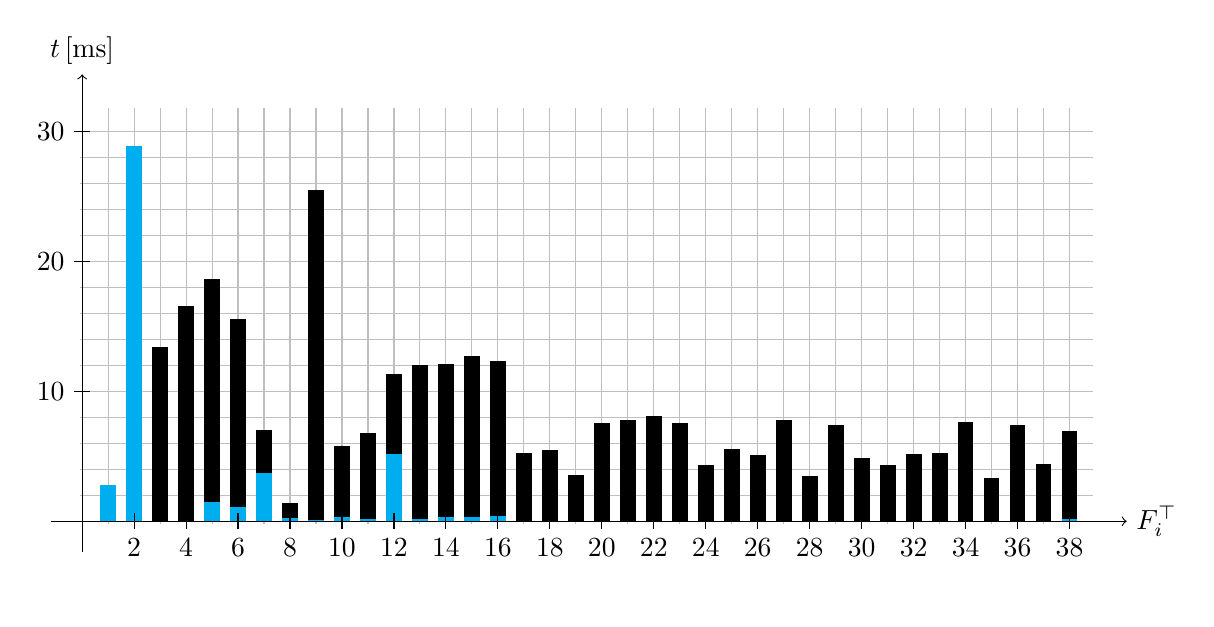
\begin{tikzpicture}[scale=0.33]
  \draw[color=lightgray] (-0.1, -0.1) grid (38.9, 15.9);
  \tikzstyle{color1}=[color=cyan]

  \def\nocachevalues{{
     2.6410,
    28.5100,
    13.3869,
    16.5449,
    18.6330,
    15.5669,
     7.0220,
     1.4099,
    25.5279,
     5.8319,
     6.8040,
    11.3669,
    11.9970,
    12.0990,
    12.6920,
    12.3380,
     5.2409,
     5.4859,
     3.5239,
     7.5699,
     7.7840,
     8.0809,
     7.5949,
     4.2960,
     5.5909,
     5.1359,
     7.8219,
     3.4979,
     7.3950,
     4.8370,
     4.3480,
     5.1550,
     5.2339,
     7.6390,
     3.3230,
     7.3960,
     4.4110,
     6.9430}}

  \def\cachevalues{{
     2.7799,
    28.8550,
     0.0019,
     0.0019,
     1.4799,
     1.0950,
     3.6849,
     0.2480,
     0.0989,
     0.3180,
     0.2019,
     5.1459,
     0.1980,
     0.3459,
     0.3060,
     0.4390,
     0.0049,
     0.0020,
     0.0029,
     0.0029,
     0.0030,
     0.0300,
     0.0309,
     0.0019,
     0.0029,
     0.0039,
     0.0029,
     0.0020,
     0.0030,
     0.0019,
     0.0040,
     0.0019,
     0.0030,
     0.0029,
     0.0029,
     0.0020,
     0.0019,
     0.2120}}

  \foreach \x in {1,2,3,4,5,6,7,8,9,10,11,12,13,14,15,16,17,18,19,20,21,22,23,24,25,26,27,28,29,30,31,32,33,34,35,36,37,38}
    \pgfmathparse{\nocachevalues[\x - 1] / 2}
    \edef\nocachevalue{\pgfmathresult}
    \draw[line width=0.2cm] (\x, 0) -- (\x, \nocachevalue);

  \foreach \x in {1,2,3,4,5,6,7,8,9,10,11,12,13,14,15,16,17,18,19,20,21,22,23,24,25,26,27,28,29,30,31,32,33,34,35,36,37,38}
    \pgfmathparse{\cachevalues[\x - 1] / 2}
    \edef\cachevalue{\pgfmathresult}
    \draw[line width=0.2cm, color1] (\x, 0) -- (\x, \cachevalue);

  \draw[->] (-1.2, 0) -- (40.2, 0) node[right] {$\ma{F}^{\top}_i$};
  \draw[->] (0, -1.2) -- (0, 17.2) node[above] {$t \left[\mathrm{ms}\right]$};

  \foreach \y in {1,2,3}
    \pgfmathtruncatemacro{\label}{10 * \y}
    \draw (0.3, 5*\y) -- (-0.3, 5*\y) node[left] {\label};

  \foreach \x in {1,2,3,4,5,6,7,8,9,10,11,12,13,14,15,16,17,18,19}
    \pgfmathtruncatemacro{\label}{2 * \x}
    \draw (2*\x, 0.3) -- (2*\x, -0.3) node[below] {\label};

  \fill[white] (0, -3) rectangle (1, -2) node {};  % Abstand nach unten

\end{tikzpicture}
% Erstelle Legende.
\begin{tabular}{llllllll}
  \toprule
  1. $\gls{M}_{00}$ & 2. $\mathrm{box}$ & 3. $\mathrm{box}_x$ & 4. $\mathrm{box}_y$ & 5. $\hat{x}$ & 6. $\hat{y}$ & 7. $\mathrm{ecc}$ & 8. $\mathrm{dia}$\\
  9. $\mathrm{ext}$ & 10. $\gls{hu}_1$ & 11. $\gls{hu}_{2}$ & 12. $\gls{hu}_{3}$ & 13. $\gls{hu}_{4}$ & 14. $\gls{hu}_{5}$ & 15. $\gls{hu}_{6}$ & 16. $\gls{hu}_{7}$\\
  17. $\gls{eta}^{\prime}_{02}$ & 18. $\gls{eta}^{\prime}_{11}$ & 19. $\gls{eta}^{\prime}_{20}$ & 20. $\gls{lambda}_1$ & 21. $\gls{lambda}_2$ & 22. $\mathrm{axis}_1$ & 23. $\mathrm{axis}_2$ & 24. $\gls{mu}_{02}$\\
  25. $\gls{mu}_{03}$ & 26. $\gls{mu}_{11}$ & 27. $\gls{mu}_{12}$ & 28. $\gls{mu}_{20}$ & 29. $\gls{mu}_{21}$ & 30. $\gls{mu}_{30}$ & 31. $\gls{eta}_{02}$ & 32. $\gls{eta}_{03}$\\
  33. $\gls{eta}_{11}$ & 34. $\gls{eta}_{12}$ & 35. $\gls{eta}_{20}$ & 36. $\gls{eta}_{21}$ & 37. $\gls{eta}_{30}$ & 38. $\mathrm{ori}$ & & \\
  \bottomrule
\end{tabular}

\caption[Laufzeitverteilung einer Merkmalsextraktion]{Laufzeitverteilung einer Extraktion aller $38$ Form-Merkmale einer \gls{SLIC}-Segmentierung mit $800$ Regionen.
Die schwarzen Balken kennzeichen die einzelnen Berechnungskomplexitäten der Merkmale.
Die blauen Balken hingegen demonstrieren den Laufzeitgewinn mittels Caching bei der Berechnung aller Merkmale.
Es zeigt sich, dass bereits nach der Berechnung des zweiten Merkmals ein deutlicher Geschwindigkeitsgewinn zu vernehmen ist.}
\label{fig:merkmals_caching}
\end{figure}


Viele der $38$ ermittelten Merkmale werden über bereits definierte Merkmale beschrieben.
So bauen insbesondere die Momente sukzessive über die zusätzlichen Stufen der Invarianz aufeinander auf.
Weiterhin erfordern Merkmale wie die Orientierung oder die Exzentrizität gleichermaßen die Berechnung der translationsinvarianten Momente sowie dessen Kovarianzmatrix.
Auch bei Merkmalen, die nicht über die Momente beschrieben sind, wie \zB{} die Berechnung des minimalen Hüllkörpers und der relativen Schwerpunktskoordinaten, lassen sich Gemeinsamkeiten in der Berechnung wiederfinden, \zB{} über die Eckpunktkoordinaten des Hüllkörpers.
Obwohl eine Berechnung aller Merkmale aufgrund der stetigen Wiederverwertung der Daten redundant erscheint und die Menge der zu benutzenden Merkmale für ein spezifisches Problem auf eine Untermenge reduziert werden sollte (\vgl{} Kapitel~\ref{merkmalsselektion}), zeigt es sich dennoch als lohnenswert, alle bereits errechneten Daten für die weiteren Berechnungen zu cachen.
Abbildung~\ref{fig:merkmals_caching} illustriert dabei den enormen Laufzeitgewinn gegenüber einer Berechnung ohne Verwendung eines Caches.
Es ist jedoch anzumerken, dass der Laufzeitgewinn mit den Kosten eines erhöhten Speicheraufwands verbunden ist.
